\begin{savequote}[75mm]
Not only is the Universe stranger than we think, it is stranger than we can think
\qauthor{Werner Heisenberg}
\end{savequote}


\chapter{Physics behind the LHCb experiment }
\label{chapter:physics}
This chapter is dedicated to providing a brief introduction to the physics of LHCb. It starts by presenting the fundamental concept of symmetries in physics, including the particular type of discrete symmetries and its consequence, then the Standard Model of particle physics is briefly described. 

\section{Symmetries in physics}
Until the 20th-century, principles of symmetry played a little role in theoretical physics. The ancient Greeks were fascinated by the symmetries of objects and believed that these would be mirrored in the structure of nature. Still, they did not manage to associate those symmetries with any deterministic law of physics. Instead, symmetry was a critical component that inspires several architects designing the most stunning and recognizable buildings, and even recently, psychologies proved that symmetrical faces are more attractive \cite{faces}. 
In one of the most important book of all time "Philosophiæ Naturalis Principia Mathematica" \cite{newton} 
Newton postulated that laws of mechanics incorporate symmetry principles, notably the principle of equivalence of inertial frames, or Galilean invariance. These symmetries implied conservation laws. Although these conservation laws, especially those of momentum and energy, were regarded to be of fundamental importance. These conservation laws were seen as consequences of the dynamical laws of nature rather than as consequences of the symmetries that underlay these laws.  

This status had dramatically changed at the beginning of the 20 century when Emmy Noether proved her famous theorem relating continuous symmetry and conservation laws.
This theorem states that due to the invariance of physics laws under spatial transformations, momentum is conserved due to time, translational invariance energy is conserved, and due to the invariance under a change in phase of the wave functions of charged particles electric charge is conserved. Precisely speaking, asymmetry is a mathematical operation that leaves the system invariant. 
From the moment of this paper publication onwards, physics can be defined as the science that studies fundamental symmetries and the mechanism of the symmetries breaking.  

In Quantum Mechanics, symmetries are mostly discreet and satisfied if an operator commutes with the Hamiltonian. If a discrete symmetry holds, it leads to a conserved quantum number and a selection rule for the transitions between different states. 
Within the framework of particle physics, there are three fundamental symmetries $P$, $C$, and $T$; those symmetries are shown in figure \ref{fig:CPT}

A parity transformation $P$ is an inversion of the spatial coordinates of a system and changing the helicity of the particle. Namely the eigenfunction of the parity operator $  \hat{P}$ satisfy the condition: 

\begin{equation}
    \hat{P}~ \ket{\Psi, \vec{r}} = \ket{\Psi, - \vec{r}} = p \ket{\Psi, \vec{r}}  
\end{equation}
Where $p$ is an eigenvalue of the $ \hat{P}$ operator and $\ket{\Psi}$ its eigenstate. A second application of the $\hat{P}$ transforms the $\ket{\Psi}$ to its initial state, therefore the $p$ must be equal to $\pm 1$, and by convention for fermions $p=1$.  


Time transformation $T$ reverse the time direction of a process, and the charge conjugation $C$ changes the sign of the quantum numbers, transforming particles into antiparticles keeping their helicity. The eigenvalues of the  charge conjugation operator $\hat{C}$ can be expressed in the following form:
 

\begin{equation}
    \hat{C}~ \ket{particle} = \ket{anti~ particle} = c \ket{particle}  
\end{equation}

Where $c$ is an eigenvalue of the $ \hat{C}$ operator, and similarly to the $\hat{P}$ operator's eigenvalues can have one of $\pm 1$ value.   

The strong and electromagnetic interactions are invariant under each of $C$, $P$, and $T$ symmetries.  The combination of $CPT$ is an exact symmetry of any interaction described by the Lorenz invariant quantum field theory. This phenomenon is described within the theory of  $CPT$ theorem \cite{CPT_theorm}.
It is observed that $C$ and $P$ are not symmetries held by the weak interactions: the weak charged currents couple exclusively to left-handed fermions and right-handed anti-fermions, and hence maximally violate $C$ and $P$ symmetries individually. The combined $CP$ operation transforms a left-handed fermion into a right-handed anti-fermion, and hence it could be expected that the $CP$ symmetry is the one that is held by the weak interactions. This statement was valid until 1964 when the group working on neutral kaons decays discovered that this is not a case, \cite{CPV_kaons}. 


\begin{figure}
\centering
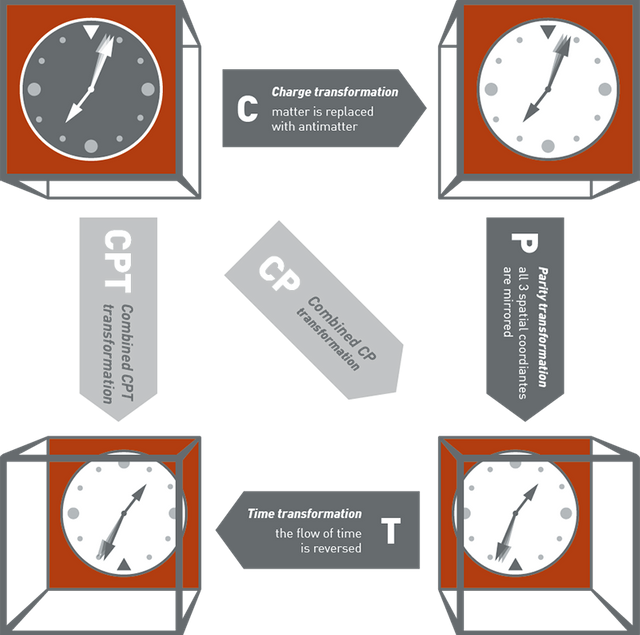
\includegraphics[scale=0.6]{figures/CPT.png}
\caption{Symmetries in particle physics. Each arrow represents a different or combination of $C$, $P$, $T$ symmetries and its influence on a system. Figure taken from \cite{CPT}
\label{fig:CPT}}
\end{figure}





\subsection{Group Theory}
This subsection is dedicated to providing a brief introduction to Group Theory, which is a branch of mathematics that was developed to studying symmetries. This section reviews some of the properties of them.

A Group $G$ is an abstract set of elements, which can be finite or infinite, with defined operator $(\cdot)$ on it, which obeys:

\begin{itemize}
    \item Closure: $\forall u,v \in G, u\cdot v \in G$
    \item Associativity: $\forall u,v,w \in G u \cdot (v \cdot w ) = (u \cdot v) \cdot w$
    \item Neutral element:  $\exists I \in G, u \cdot I = I \cdot u = u, \forall u \in G$
    \item Inverse element:  $\exists u \in G, \exists u^{-1} \in G, u \cdot u^{-1} = I$
\end{itemize}

Group G is called Abelian or commutative if also the following axiom is satisfied:
\begin{itemize}
    \item Commutativity $\forall u,v \in G u \cdot v = v \cdot u$
\end{itemize}

In elementary particle physics, the most common groups are of the type of $U(n)$, which is a collection of all unitary $n\times n$ matrices \footnote{A unitary matrix is one whose inverse is equal to its transpose conjugate $U^{-1}=U^\dagger$}. The second type of group used to construct the Standard Model is a Super Unitary group $SU(n)$. In addition to the $U(n)$, $SU(n)$ requires the matrix determinant is equal to 1. 
A group of matrices can represent every group, thus for every element $u$ there is corresponding matrix $M_u$, which needs to fulfill all axioms listed above. 

As a concrete example let consider a group of real, orthogonal \footnote{An orthogonal matrix is an matrix whose inverse is equal to its transpose: $O^{-1} = O^{T}$} $n\times n$ matrices of determinant 1, this group called $SO(n)$ and can represent all rotation is a space of $n$ dimensions. For $n=3$, group $SO(3)$  describes rotational symmetry of our word, which according to the Noether's theorem is equivalent to the conservation of angular momentum \cite{griffiths}. 

\section{Standard Model for elementary particle}
\label{sec:SM}

The Standard Model (SM) is a Quantum Field Theory that describes properties of the elementary particles and the electromagnetic, weak, and strong interactions. It has been experimentally validated on numerous occasions,
making very accurate predictions. However, it is an incomplete theory since it does not include the gravity interaction and does not explain the dark matter and dark energy, the neutrino masses, nor the matter-antimatter asymmetry of the Universe.

This theory was built to model the particle interaction observed in nature. Using this framework, one can obtain predictions for physical phenomena by calculating transmission probability from an initial state $\bra{i, i'}$ to a given final state$\ket{k, k' }$. These calculations are performed using Quantum Field Theory tools such as expansions of a path integral into a power series, which can be visualized using Feynman diagrams (one diagram per term). Each term in those series can be interpreted as a particular interaction process. 

According to the Standard Model, the whole space is filled with different types of field, and the excitation of those fields are what can be interpreted as particles, the visualization of properties of elementary particles are shown in figure \ref{fig:SM} . The matter is built by twelve particles called fermions \footnote{And their corresponding antiparticles}, which has a half-integer spin, and they have to obey the Pauli exclusion principle. The interactions between fermions are perceived as an exchange of integer spin particles called bosons. 
None of them are known to have any underlying substructure.
All fermions can be further split into two groups: quarks and leptons. This split is driven by the interaction in which a particular fermion can involve. 


The fundamental properties of the Standard Model of Particle Physics the fact that it is based on the following symmetry groups:

\begin{equation}
    SU(3)_C \times SU(2)_L \times U(1)_Y
\end{equation}



Where the term $SU(3)_C$ is responsible for the strong interactions, which are mediated by eight massless gluons and occurs between quarks, those interactions are described by a theory called Quantum Chromodynamic (QCT).  Only the quarks can carry color charge, which allows them to interact via the strong interaction. Quarks occur in six flavors up $u$,  down $d$, charm $c$, strange $s$, top $t$ and beauty $b$.  Due to the unique nature of the strong interaction, in which the mediators of the force, the gluons, carry the same color charge that they mediate, quarks are \footnote{This happens for all quarks besides the top quark, which lifetime is too short to combine with other quarks to form hadrons} glued to the other quarks to form colorless particle composition called hadrons. 

Depending on the number of quarks they are made of, hadrons are classified to mesons (composed of $q\bar{q}$ pair), baryons (with three quarks combining all the colors) and exotic hadrons composed of four and five quarks, which has been recently discovered and reported by the LHCb collaboration \cite{pentaquarks}.  



\begin{figure}
\centering
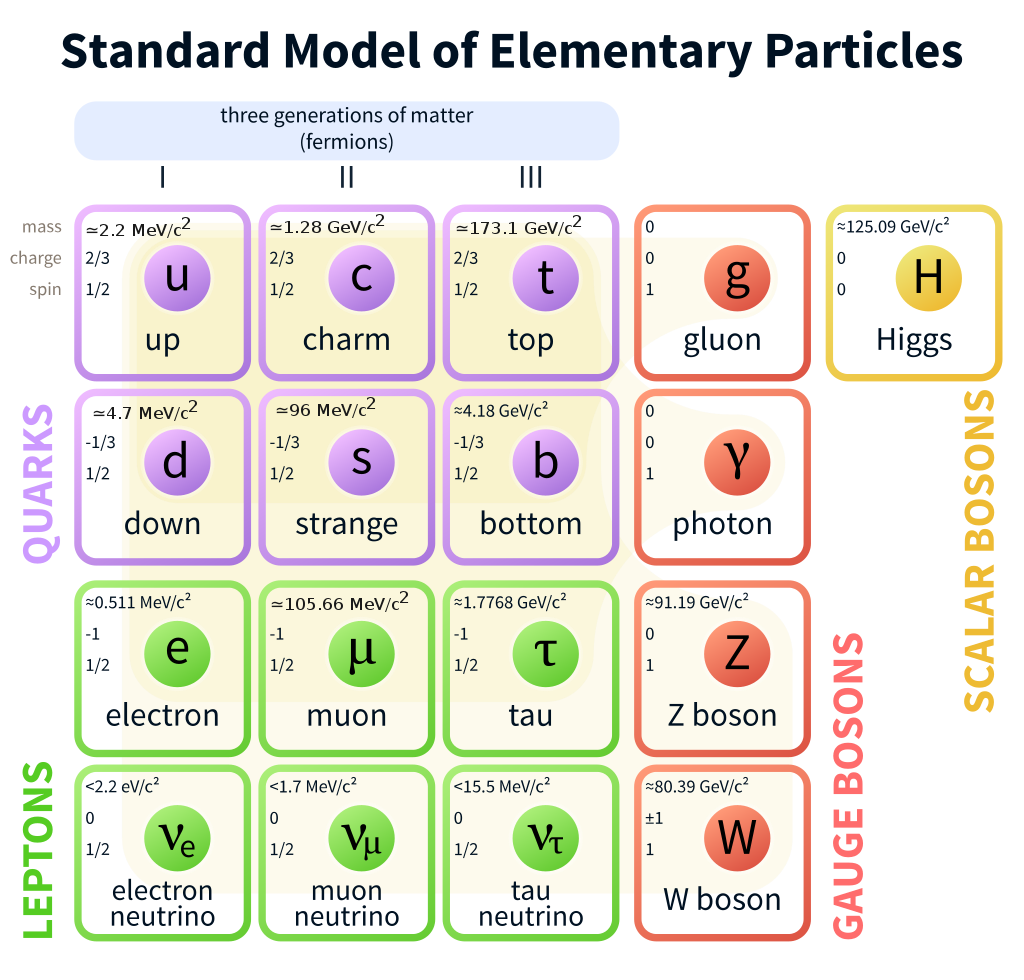
\includegraphics[scale=0.5]{figures/SM.png}
\caption{Illustration of the fundamental particles in the Standard Model and their properties. The fermions organized in three generations (denoted by I, II, and III) comprise of quarks preseted as the purple squares and leptons as the green squares. The bosons consist of the gauge bosons denoted in red, and the scalar Higgs boson indicated by the yellow square. 
\label{fig:SM}}
\end{figure}

\section{Weak interactions and CKM matrix}

The $ SU(2)_L \times U(1)_Y$ symmetry describes the gauge group of electroweak interactions. Those interactions are carried by four bosons, namely $W^{\pm}$, $Z$, and the $\gamma$.  The first two of them mediate the weak interaction, and $\gamma$ is responsible for carrying electromagnetic interaction. One of the key features of the weak interaction is the experimental observation that they couple to the left-handed particles only, which revealed as a maximum violation of the parity. Another unique feature of the weak forces is the mixing between different quarks families, which is understood as the quark mass eigenstates are not the same as the weak eigenstates. The Cabibbo-Kobayashi-Maskawa (CKM) matrix relates the weak eigenstates,  ($d\prime$,$s\prime$,$b\prime$), with the mass eigenstates, ($d$,$s$, $b$), and is written as:

\begin{equation}
\label{eq:ckm}
  \begin{bmatrix}  d^\prime  \\  s^\prime  \\  b^\prime  \end{bmatrix} = \begin{bmatrix} V_{ud} & V_{us} & V_{ub} \\ V_{cd} & V_{cs} & V_{cb} \\ V_{td} & V_{ts} & V_{tb} \end{bmatrix} \begin{bmatrix}  d  \\  s  \\  b  \end{bmatrix}
\end{equation}


where the $3 \times 3$ unitary matrix $V_{CKM}$ is known as the Cabibbo-Kobayashi-Maskawa (CKM) quark mixing matrix\cite{}\cite{}. The magnitude of each element in $V_{CKM}$ represents the coupling strength of the quarks in the subscript to the weak field $W^{\pm}$ boson.  One of the properties of such a matrix is the possibility to fully describe its transformation properties by three Euler angles and one complex phase angle. Analysis of the value of this phase is vital due to it is not invariant under time reversal $R$ symmetry, which implies violation of Charge-Parity $CP$ symmetry if its value is not zero:

\begin{align} V_{CKM}  &= \begin{bmatrix} 1 & 0 & 0 \\ 0 & c_{23} & s_{23} \\ 0 & -s_{23} & c_{23} \end{bmatrix}
 \begin{bmatrix} c_{13} & 0 & s_{13}e^{-i\delta_{13}} \\ 0 & 1 & 0 \\ -s_{13}e^{i\delta_{13}} & 0 & c_{13} \end{bmatrix}
 \begin{bmatrix} c_{12} & s_{12} & 0 \\ -s_{12} & c_{12} & 0 \\ 0 & 0 & 1 \end{bmatrix} \nonumber \\ 
 & = \begin{bmatrix} c_{12}c_{13} & s_{12} c_{13} & s_{13}e^{-i\delta_{13}} \\
 -s_{12}c_{23} - c_{12}s_{23}s_{13}e^{i\delta_{13}} & c_{12}c_{23} - s_{12}s_{23}s_{13}e^{i\delta_{13}} & s_{23}c_{13}\\
 s_{12}s_{23} - c_{12}c_{23}s_{13}e^{i\delta_{13}} & -c_{12}s_{23} - s_{12}c_{23}s_{13}e^{i\delta_{13}} & c_{23}c_{13} \end{bmatrix}
\end{align}
where $c_{ij} =\cos(\theta_{ij})$, $s_{ij} =\sin(\theta_{ij})$,  $\theta_{ij}$ are the mixing angles, and $\delta_{13}$ is a complex phase. Angle $\theta_{12}$ is called Cabbibo angle, which was introduced in 1963 when only two generation of quarks were known \cite{cabibbo}. 


One of the parametrizations of the $V_{CKM}$, that is convenient to present the hierarchical structure of its parameters is called Wolfenstein \cite{wolfenstein} parametrization:.

\begin{equation}
\label{eq:wolfenstein}
   V_{CKM} =  \begin{bmatrix} 1-\tfrac{1}{2}\lambda^2 & \lambda & A\lambda^3(\rho-i\eta) \\
 -\lambda & 1-\tfrac{1}{2}\lambda^2 & A\lambda^2 \\
 A\lambda^3(1-\rho-i\eta) & -A\lambda^2 & 1  \end{bmatrix} + O(\lambda^4).
\end{equation}


Experimentally, it is found that the mixing between mass and weak eigenstates is relatively small in the quark sector. Based on current knowledge \cite{CKMFitter}, the values of $V_{CKM}$ parameters are:
\begin{itemize}
\item $\lambda=0.224837^{+0.000251}_{-0.000060}$,
 \item  $A= 0.8235^{+0.0056}_{-0.0145]}$, 
 \item  $\rho=0.1569^{+0.0102}_{-0.0061}$,
 \item  $\eta=0.3499^{+0.0079}_{-0.0065}$.
\end{itemize}

 Therefore each of the mixing angles, represented as an off-diagonal element \ref{eq:ckm}, is small, and the CKM matrix is approximately diagonal, see figure \ref{fig:ckm_magnitudes}. Therefore, processes that involve off-diagonal elements of the CKM matrix, those that change the generation of the quarks are Cabibbo-suppressed with respect to those on the diagonal, which are referred to as Cabibbo-favoured.



\begin{figure}[h]
\centering
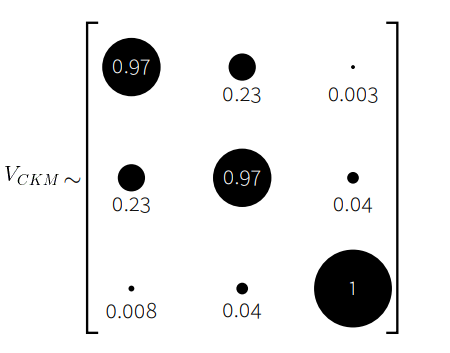
\includegraphics[scale=0.5]{figures/ckm_structure.PNG}
\caption{Hierarchy of the $V_{CKM}$ matrix elements. The numbers are approximate to illustrate the relative magnitudes of the elements.  
\label{fig:ckm_magnitudes}}
\end{figure}



 The consequence of the fact that there are three quarks families only is unitarity of the $V_{CKM}$ matrix. This property gives a series of constraints between different elements of the  $V_{CKM}$ matrix that can be tested experimentally. These constraints impose the following relations:

\begin{equation}
\label{eq:unitary}
\begin{split}
        V_{1j}^{*}V_{1k} +  V_{2j}^{*}V_{2k} +  V_{j3}^{*}V_{3k} = \delta_{jk} \\
        V_{j1}^{*}V_{k1} +  V_{j2}^{*}V_{k2} +  V_{j3}^{*}V_{k3} = \delta_{jk} 
\end{split}
\end{equation}

Those six relations, summarized by equation \ref{eq:unitary}, can be visualized as triangles in the complex plane.  The most popular to study is the triangle with  $j=b$ and $k=d$. It drew attention due to having all sides of the same order of magnitude.  This triangle can be completely constructed by a single apex:
\begin{equation}
   (\overline{\rho}, \overline{\eta}) =- \frac{V_{ub}^{*}V_{ud}}{V_{cb}^{*}V_{cd}}
\end{equation}
while the remaining apexes are $(0,0)$ and $(0,1)$.  
The angles of this unitary triangle denoted as $\alpha, \beta, \gamma$ are defined as follow: 

\begin{align*}
   \alpha &= arg\left( \frac{V_{tb}^{*}V_{td}}{V_{ub}^{*}V_{ud}} \right), & 
   \beta &=  arg\left( \frac{V_{cb}^{*}V_{cd}}{V_{tb}^{*}V_{td}} \right), &
   \gamma &= arg\left( \frac{V_{ub}^{*}V_{ud}}{V_{cb}^{*}V_{cd}} \right) 
\end{align*}



\begin{figure}[h]
\centering
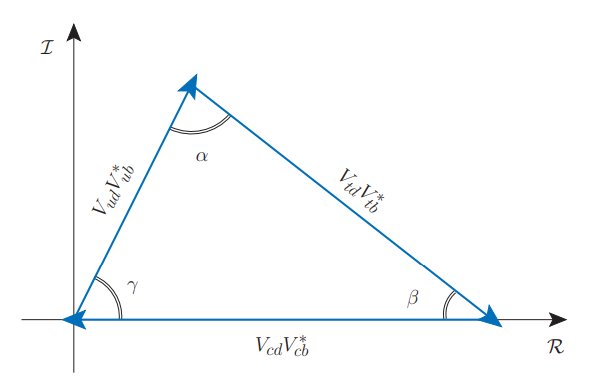
\includegraphics[scale=0.8]{figures/Unitary_triangle.PNG}
\caption{Visualization of one of the unitary triangles of the $V_{CKM}$ matrix. Definition of the angles $\alpha, \beta, \gamma$ can be found in text.   
\label{fig:triangle}}
\end{figure}

The values of those angles cannot be predicted using the Standard Model framework. Instead, they can be measured experimentally. Any possible discrepancy in relation \ref{eq:unitary} may indicate a contribution from physics beyond the Standard Model. Figure \ref{fig:traingle} shows the overall status of the CKM unitary triangle in the $\overline{\rho}, \overline{\eta}$ plane, with a global fit to the apex. Within the current experimental uncertainties, there are no significant deviations from the Standard Model predictions. 

\begin{figure}
\centering
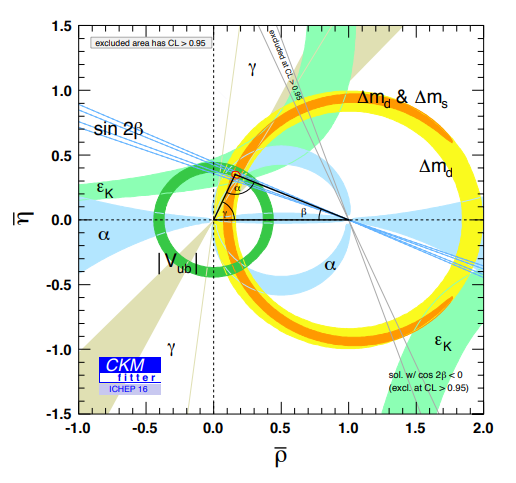
\includegraphics[scale=0.6]{figures/Unitary_triangle_constrains.PNG}
\caption{Overlapping constraints of the CKM unitary triangle. The red dashed area indicates global fit of the CKM apex with 68\% confidence interval. Figure adopted from \cite{CKMFitter}.
\label{fig:triangle}}
\end{figure}


\section{Neutral Meson Mixing and $CP$ violation}

One of the promising channel that can be used in order to measure the $CP$ violation and it is a manifestation the fact that the mass eigenstates are not the same as the weak eigenstates is the phenomenon of flavor oscillation in neutral mesons ($K^0$, $D^0$, $B^0$, and $B^0_ s$ ). 
Those mixing processes can be described by the so-called box diagram presented in figure \ref{fig:Mixinig}. 


\begin{figure}
\centering
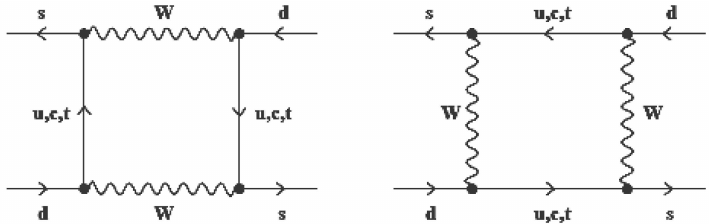
\includegraphics[scale=0.9]{figures/Box-diagrams-depicting-K-0-K-0-mixing.png}
\caption{Box diagrams illustrating the mixing of $K^{0}$ mesons. In both cases virtual $W$ bosons
and quarks connect the four vertexes. Figure adopted from \cite{Mixing}.
\label{fig:Mixinig}}
\end{figure}


The mass eigenstates are written as a superposition of flavor eigenstates:
\begin{equation}
    \begin{split}
        \ket{M_L} = p \ket{M} + q \ket{\overline{M}} \\
        \ket{M_H} = p \ket{M} - q \ket{\overline{M}} \\
    \end{split}
\end{equation}
 where $p$ and $q$ are complex numbers satisfying the normalization condition $|p|^{2}+|q|^{2} = 1$. 
 The evaluation of this system is determined by the non-hermitian Hamiltonian, given as: 

\begin{equation}
\label{eq:mixing_hamiltonian}
    \mathcal{H}  = \textbf{M} - \frac{i}{2} \textbf{\Gamma}
\end{equation}


where $\textbf{M}$ and $\textbf{\Gamma}$ are the mass and width matrices, respectively, defined as: 

\begin{align}
    \textbf{M} &= \left( \begin{matrix} M_{11} & M_{12}  \\ M_{12}^{*} & M_22 \end{matrix} \right), & 
    \textbf{\Gamma} &=  \left( \begin{matrix} \Gamma_{11} & \Gamma_{12}  \\ \Gamma_{12}^{*} & \Gamma_22 \end{matrix} \right) 
\end{align}

The Hamiltonian of the process, equation \ref{eq:mixing_hamiltonian}, is not hermitian, thus ensures that the neutral meson may eventually decay. The on-diagonal elements of both $\textbf{M}$ and $\textbf{\Gamma}$ matrixes are the same due to $CPT$  theorem, and if the off-diagonal elements are equal to zero the meson states are degenerated and the mixing would not occur. Moreover both  $\textbf{M}$ and $\textbf{\Gamma}$ are hermitian. 
The time evolution of the flavor eigenstates obeys the time-dependent Schrodinger equation:

\begin{align}
\label{eq:time dependent hamiltonian}
\centering
    i\frac{d}{dt} \left(\begin{matrix} \ket{M(t)}  \\ \ket{\overline{M}(t)} \end{matrix}  \right) 
    &= \mathcal{H} \left(\begin{matrix} \ket{M(t)}  \\ \ket{\overline{M}(t)} \end{matrix}  \right) \\
    i\frac{d}{dt} \left(\begin{matrix} \ket{M(t)}  \\ \ket{\overline{M}(t)} \end{matrix}  \right) 
    &=\left( \begin{matrix} M_{11} - i\frac{1}{2}\Gamma_{11} & M_{12} -i\frac{1}{2}\Gamma_{11} \\ M_{12}^{*} - i\frac{1}{2}\Gamma_{12}^{*} & M_22-i\frac{1}{2}\Gamma_{22} \end{matrix} \right) \left(\begin{matrix} \ket{M(t)}  \\ \ket{\overline{M}(t)} \end{matrix}  \right) 
\end{align}

The solution of the equation \ref{eq:time dependent hamiltonian} is a pair of eigenvalues given by:

\begin{align}
\centering
    v_{1} &= \left( \begin{matrix} p  \\ q \end{matrix} \right), & 
    v_{2} &=  \left( \begin{matrix} p \\ -q \end{matrix} \right) 
\end{align}

Those eigenvalues allows to diagonalize the hamiltonian: 

\begin{align}
   Q\mathcal{H}Q^{-1} &= P =  \left( \begin{matrix} M_{L} - \frac{i}{2}\Gamma_{L} & 0  \\ 0 &  M_{H} - \frac{i}{2}\Gamma_{H}  \end{matrix} \right) 
\end{align}
where $Q$ is a matrix composed of vertically stacked $v_1$ and $v_2$, and $P$ is a auxiliary matrix introduced to simplify notation. 
Using mentioned notation the time evolution of the flavor states can be written as:

\begin{align}
\label{eq:time_evaluation}
  \left(\begin{matrix} \ket{M(t)}  \\ \ket{\overline{M}(t)} \end{matrix}  \right) 
  = QPQ^{-1} \left(\begin{matrix} \ket{M}  \\ \ket{M} \end{matrix}  \right) 
  = \left(\begin{matrix} g_{+}(t) &  \frac{q}{p}g_{-}(t)  \\  \frac{p}{1}g_{-}(t)  & g_{+}(t)  \end{matrix}\right) 
  \left(\begin{matrix} \ket{M}  \\ \ket{M} \end{matrix}  \right)   
\end{align}

where the parameters $g_{\pm}$ are given :

\begin{align}
    g_{+} &= e^{-imt}e^{\Gamma \frac{t}{2}} \left[ \cosh(\frac{\Delta \Gamma t}{4})\cos(\frac{\Delta M t}{2})  - i\sinh(\frac{\Delta \Gamma t}{4})\sin(\frac{\Delta M t}{2})  \right] \\ 
    g_{-} &= e^{-imt}e^{\Gamma \frac{t}{2}} \left[ \sinh(\frac{\Delta \Gamma t}{4})\cos(\frac{\Delta M t}{2})  - i\cosh(\frac{\Delta \Gamma t}{4})\sin(\frac{\Delta M t}{2})  \right]   
\end{align}
and $m = \frac{1}{2}(M_{L}+M_H)$, $\Gamma =  \frac{1}{2}(\Gamma_{L}+\Gamma_{H})$, $\Delta M = M_{H}- M_{L}$, $ \Delta \Gamma =(\Gamma_{L}-\Gamma_{H})$.

The equation \ref{eq:time_evaluation} allows expressing the probability of mixing from particle to their antiparticle and vise-versa. Those probabilities are given by 

\begin{align}
\label{eq:mixing_prob}
|\bra{\overline{M}} \mathcal{H} \ket{M}|^{2} = \left|\frac{q}{p}\right|^{2} |g_{-}(t)| = \frac{e^{\Gamma t}}{2} \left|\frac{q}{p}\right|^{2}  \left[ \cosh(\frac{\Delta \Gamma t}{2})\cos(\Delta M t) \right] \\ 
|\bra{M} \mathcal{H} \ket{\overline{M}}|^{2} = \left|\frac{p}{q}\right|^{2} |g_{-}(t)| = \frac{e^{\Gamma t}}{2} \left|\frac{p}{q}\right|^{2}  \left[ \cosh(\frac{\Delta \Gamma t}{2})\cos(\Delta M t) \right]
\end{align}

The equation \ref{eq:mixing_prob} clearly indicates that the mass difference between light and heavy states drives the mixing frequency. It is also important to analyze ratio $\frac{p}{q}$. If it differ from 1 then the mixing process violate $CP$ symmetry. The word average of this mixing parameter in $B^{0}$ is  $\frac{p}{q} = 1.0009 \pm 0.0013$ and  for $B_s$  $\frac{p}{q} = 1.0003 \pm 0.0014$ \cite{PDG}, which means the results are consistent with $CP$ symmetry. 

\section{The Baryon Asymmetry of the Universe and Sakharov conditions}

The previous sections described the combined $CP$ symmetry and discussed possible channels to study its violation. Here comes a viral question. Why do the researchers study the $CP$ violation? Why is it so crucial that even it is mentioned inside of the logo of the LHCb experiment? 

One of the answers to this question is the problem of the asymmetry of baryons with respect to anti-baryon. The current observed Universe is filled with baryons.  This observation is contradicted to the cosmological measurement, which strongly indicates that in the era of the early Universe, the matter and antimatter should have been created in equal amounts. Therefore, there must have been some process that had created the matter-antimatter asymmetry.  
In 1967 soviet physicist Sakharov postulated three conditions that have to be fulfilled in order to make baryogenesis, or in other words existence of known Universe,  possible \cite{sakharov}: 

\begin{enumerate}
    \item \textbf{Baryon number violation}.  All known perturbative processes in the Standard Mode result in equal numbers of baryons and anti-baryons. However, there are non-perturbative electroweak processes that can produce baryons without anti baryons \cite{bayron_number_violation}. 
    \item \textbf{$C$ and $CP$ violation}. Violation of these symmetries are required even if there are processes, see the first condition, that could generate more baryon that anti-baryon an opposing process would generate an excess of anti-baryons, so the net baryon number of the system would still remain the same.
    \item \textbf{Departure from thermal equilibrium}. Baryogenesis cannot occur at thermal equilibrium; otherwise, the inverse of this process will occur at the same rate, and a net asymmetry will not be generated.
\end{enumerate}

The first condition is fulfilled by one of the default property of the Standard Model that it requires the baryon minus lepton number to be conserved, but it does not have any restriction on conservation of an individual of this numbers.  The mechanism that would allow satisfying the third condition is the electroweak phase transition. Although, due to the mass of the Higgs boson $m_H \approx 126 GeV/c^{2}$, the phase transition would only be weakly first order and not provide a strong enough departure from thermal equilibrium \cite{phase_transiton}. 

 Within the Standard Model framework, the only source of the violation of $CP$ symmetry is the weak interactions in the quark sector. Although the known $CP$ violation in the quark sector is about ten orders of magnitude too small to explain baryogenesis, and therefore it is likely that this additional CP-violation originates in physics beyond the Standard Model. Therefore, precise comparisons of CP-violating observables and the Standard Model's predictions provide an invaluable probe of the New Physics.